%!LW recipe=pdflatex-shellescape
\documentclass[11pt]{article}

\usepackage{geometry}
\geometry{margin=0.5in}

\usepackage[utf8]{inputenc}
%\usepackage[english]{babel}

\usepackage{graphicx}
\usepackage[dvipsnames]{xcolor}
\usepackage{amsmath}
\usepackage{float}
\usepackage{natbib}
\bibliographystyle{mnras}
\setcitestyle{authoryear,open={(},close={)}}
\usepackage[hybrid]{markdown}
\usepackage{enumitem}
\setitemize{itemsep=-2pt}
\usepackage[colorlinks=true,allcolors=blue]{hyperref}
\usepackage{caption}
\usepackage{overpic}

\begin{document}

\tableofcontents
\clearpage

\section{Literature review}

\subsection{Artificial chemistries}

\subsubsection{\texorpdfstring{\cite{dittrich_artificial_2001}}{}}

\begin{markdown}

**tldr;** Comprehensive review of the field of Artificial Chemistry, the ways to define artificial chemistry systems, different characteristics and methods, various approaches, considerations when modeling living systems and key questions related to modeling specific systems.

- working hypothesis of Artificial Life research: biology can be modeled using complex systems of many interacting components, as there’s emergence of novel global behavior from local interactions that’s not predictable from the properties of its components but is rather due to their organization/function
    
- Artificial Chemistry (AC) should be able to explain the origin of evolutionary systems leading to the evolution of life
    
- AC has three main dimensions in its application: modeling (of biological/evolutionary/social systems), information processing (investigating chemical systems that perform computation), optimization (using chemical systems to find solutions to combinatorial problems)
    
- we define an AC as (S, R, A): S being the set of molecules, R the collision rules, A the algorithm (i.e., vessel where the reactions take place)
    
- set of molecules S: can be abstract symbols, character sequences, lambda-expressions, binary strings, numbers, etc.
    
- set of rules R: chemical notation describing the reactions
    
- algorithm A: simplest case is a multiset or concentration vector—can be modeled as an algorithm that draws molecules randomly, using PDEs, etc.
    
- alternative definition using the (S, I) notation: S the set and I the interactions, can be preferable if on a lattice
    
- characteristics and methods of an AC system include: the definition of molecules (explicit or implicit), reaction laws (idem), dynamics (idem), level of abstraction (analogous or abstract), constructive dynamics (if the dynamics can change over time), random chemistries (systems based on random rules/rate constants), time scale, pattern matching, spatial topology
    
- approaches: see Table~\ref{tab:dittrich2001}
    
- we can use AC systems to study living organisms as information processing units
    
- several phenomena are commonly observed in AC systems: reduction of diversity, formation of densely coupled stable networks, syntactic and semantic closure, evolution and punctuated equilibrium
    
- important questions include: what level of abstraction is appropriate? which key ingredients? how much physical/chemical knowledge to include? et cetera.

\end{markdown}

\begin{figure}[hbt]
  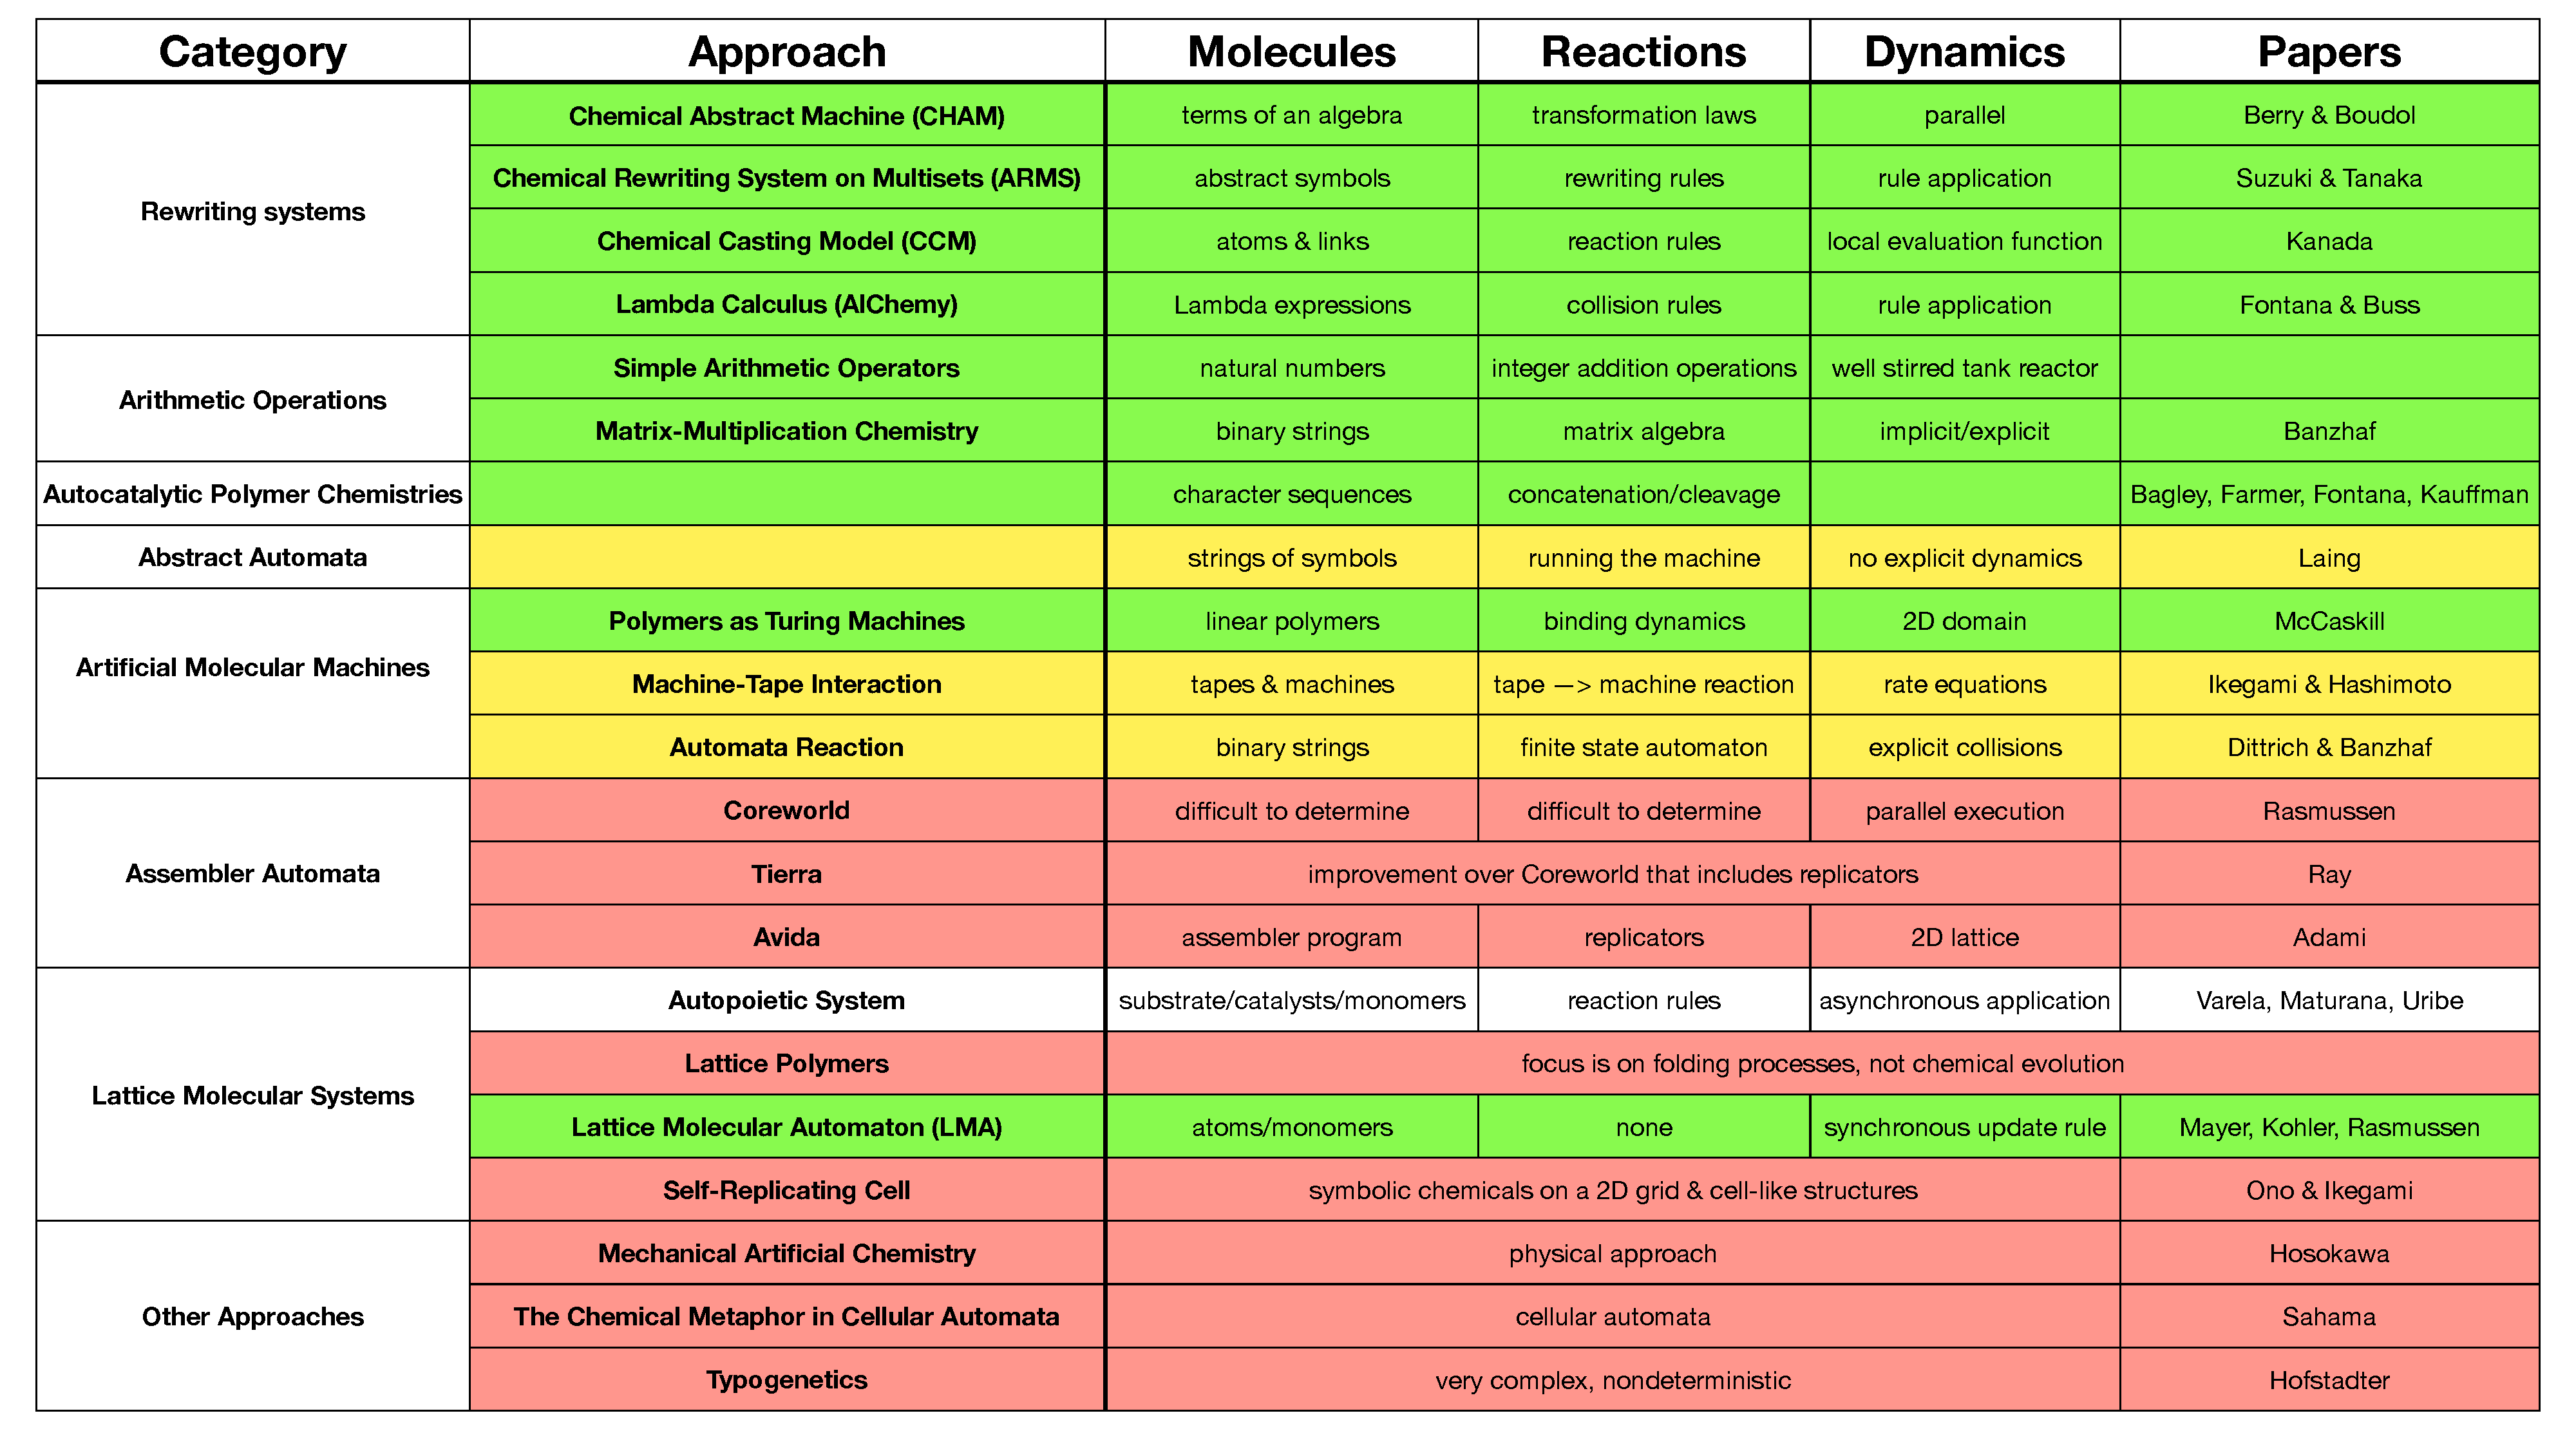
\includegraphics[width=\textwidth]{figures/dittrich2001/dittrich-table.pdf}
  \caption{Summary of approaches reviewed in \cite{dittrich_artificial_2001}. Color coding indicates closeness to the present project.}
  \label{tab:dittrich2001}
\end{figure}



\clearpage

\subsubsection{\texorpdfstring{\cite{liu_definition_2020}}{}}

\begin{markdown}

**tldr;** Provides an analysis, using an artificial chemistry system, of self-sustainability and heredity, and offers a formal definition that allows to determine whether a system is self-sustaining.

- the ability to self-sustain is central to life, but a definition of self-sustainability is missing
    
- connecting self-sustainability with heredity, another feature central to life, is another problem
    
- here the author proposes a definition of self-sustainability taking into account the chemical reaction network and the external environment, simplified as a continuous-flow stirred tank reactor (CSTR)
    
- self-sustaining can either mean: “no-intervention” (e.g., NASA definition) or “regeneration” (e.g., autopoiesis)
    
- no-intervention school: RNA amplification is self-sustaining as it can be continued indefinitely
    
- regeneration school: each molecule can be produced from the food source (RAF theory), if topologically all molecules consumed are also produced (chemical organization theory)—three issues with this latter definition (topological, defined wrt. molecules, too stringent)
    
- origin of life: would require the origin of self-sustainability and the origin of heredity—this is why we question theories of self-sustaining chemistry without heredity
    
- we define the model as a set of ODEs describing the mean field dynamics (see eq. 2)
    
- two assumptions: all molecules are uniformly distributed, all species have the same molar volume --> solution behaves like an ideal gas
    
- we can define mathematically self-sustainability wrt. the inflow f and the initial conditions xi
    
- we can define multiple concepts related to self-sustainability: trivial, self-sustaining, impossible, sequential
    
- we suggest that a self-driven CRN is irreducible self-sustaining if it satisfies the criteria for “overproduction” and “no-over-intake”
    
- moreover, if a CRS is self-sustaining, it has preliminary heredity: self-sustainability’s trigger molecule can by considered a “holistic, limited hereditary replicator”
    
- whether a system is self-sustaining also depends on the environment
	
\end{markdown}



\clearpage

\subsubsection{\texorpdfstring{\cite{virgo_complex_2016}}{}}

\begin{markdown}

**tldr;** Modeling an Artificial Chemistry system in the thermodynamically reversible regime leads to self-organization of autocatalytic cycles, and by blocking simple ACSs we get more complex ones yielding super-exponential growth

- the authors show that even very simple chemistries in the TD reversible regime can self-organize to form complex autocatalytic cycles, with the catalytic effect emerging from the network structure
    
- by suppressing the direct reaction from reactants to products, we get ACS, leading to exponential growth—exponential autocatalysis is interesting from an ool point of view as it could exist before the invention of cell membranes/compartmentalization needed to increase concentrations
    
- previous approaches: Fontana/Buss, Kauffman—but these lack TD considerations, which we reintroduce here
    
- we demonstrate that ACSs *necessarily* arise in chemistry that meets simple preconditions by blocking autocatalysis, which leads to ACSs appearing through a second-order mechanism
    
- energy “flowing downhill”, blocking simple autocatalysis yields more complex cycles, alongside bistability and oscillations—this depends on the topology of the reaction network
    
- key feature of including TD considerations in an AC system: the direction of reactions isn’t constrained, such that equilibrium will follow the principle of detailed balance
    
- here we use, as an implementation of chemical dynamics, mass-action kinetics—a well-mixed reactor where molecules collide at random and react with a probability proportional to the rate constant of the reaction—TD puts constraints on the values of these constants
    
- A-polymerization model: we use unary strings (A, AA, AAA, …) noted A1, A2, A3, …which can be thought of as non-oriented polymers with all the reactions of the form Ai+Aj-->A(i+j)
    
- we will block certain reactions, and only allow reactions in the set called R (permitted reactions)
    
- rate constants are ks (synthesis) and kd (decomposition) and are uniform
    
- mass action kinetics leads to a set of ODEs for the concentration of each species (eq. 2)
    
- the linear case: we disallow monomers from forming a dimer and conversely, but all other reactions are permitted (some autocatalytic cycles can convert monomers into dimers)—we then observe exponential growth due to ACS cycles with the distribution of polymers depending on the rate constants (see fig1)
    
- superexponential growth: if we prevent first-order autocatalysis by explicitely banning species from reacting, exponential growth still occurs through second-order mechanisms
    
- additional conclusion: non-equilibrium systems, under *some* conditions, tend not only to flow downhill but to find faster and faster ways to do it—relevant for ool research as this combinatorial explosion would mean a faster exploration of possible primitive replicators

\end{markdown}

\begin{figure}[hbt]
  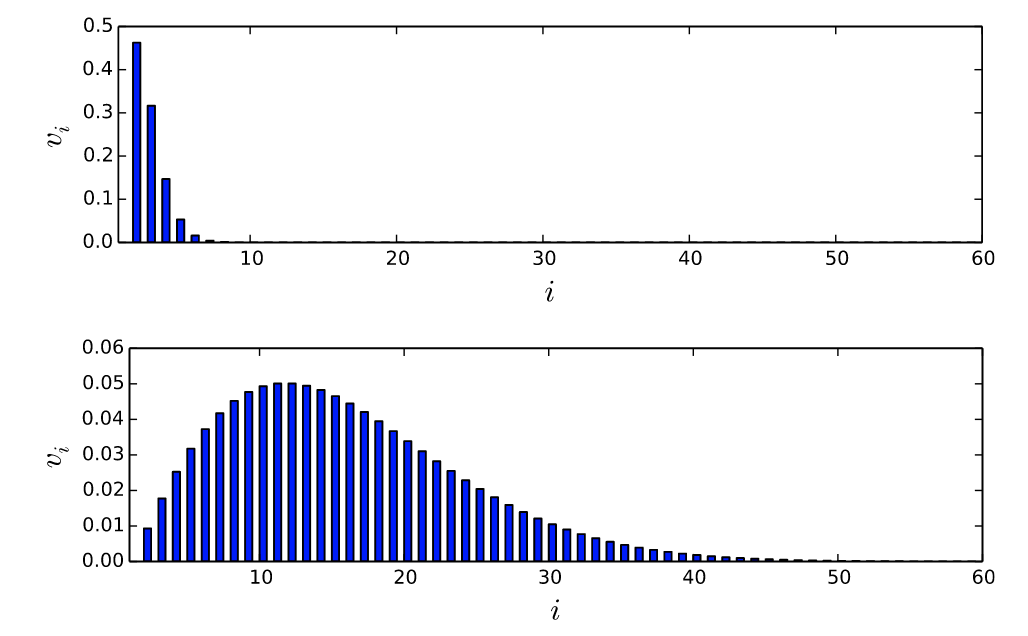
\includegraphics[width=\textwidth]{figures/virgo2016/fig1.png}
  \caption{Example of exponential growth in the linear model of \cite{virgo_complex_2016}. Top vs bottom panels display different reaction rates.}
  \label{fig:virgo2016fig1}
\end{figure}

\begin{figure}[hbt]
  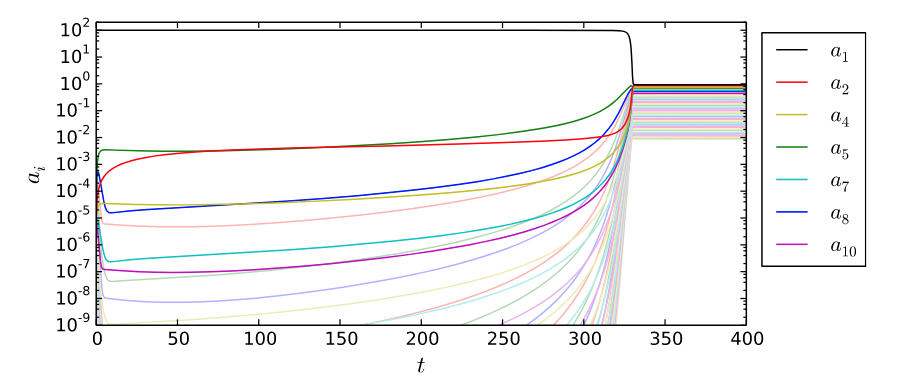
\includegraphics[width=\textwidth]{figures/virgo2016/fig2.png}
  \caption{Illustration of super-exponential growth in \cite{virgo_complex_2016} in the non-linear case when banning species.}
  \label{fig:virgo2016fig2}
\end{figure}


\clearpage

\subsubsection{\texorpdfstring{\cite{walker_universal_2012}}{}}

\begin{markdown}

**tldr;** The authors present a model of artificial chemistry that combine hydration-dehydration cycles with sequence replication on a diffusive lattice, and demonstrate that limited diffusion can provide an alternative to compartmentalization.

- the authors present a model for what was an earlier stage of evolution than e.g. refinement of preexisting enzymes (like replicase)—the model includes environmental cycles (e.g. hydration-dehydration) which coincide with different monomer/polymer diffusivity—it is also observed that polymers form cluster/aggregates
    
- we introduce the term Universal Sequence Replication (USR) to represent the possibility that prebiotic template-directed synthesis provided means for the replication of polymers, regardless of monomer sequence (i.e. replicative rate constants are sequence-independent)
    
- Kinetic Monte Carlo simulations are used to evolve populations of informational polymers, formed by spontaneous polymerization, replicated by USR and then subject to hydrolysis in a diffusion-limited environment—resulting in species diversity remaining high despite functional selection not dominating the system
    
- cycling: polymerization via spontaneous assembly and USR via template-directed synthesis occur in the hot-dry conditions whereas polymer degradation and diffusion of monomers and polymers occur in the cool-wet conditions—functional polymers only exhibit catalytic activity during the hydrated phase that promotes the folding into the active state
    
- reversible polymerization: polymers degrading into monomers are added back into the population, creating feedback between both concentrations
    
- monomer concentrations: the total number of monomeric units (e.g. nucleotides) is constant, with species labeled A and B
    
- surface confinement and limited diffusion: polymers and monomers are confined to a 2D surface, where diffusion takes place in the hydrated phase—size 64x64
    
- USR: all polymers have the same rate constant for replication
    
- emergence of a functional polymer: we explore the emergence of the first functional informational polymer, here referred to as an A-zyme, capable of synthesizing A monomers from proto-A
    
- polymer species: we choose a fixed length of RL=20
    
- spatial patterning: we observe spatial patterning of polymers that is dependent on the diffusivities, and which can be interpreted as an indirect form of cooperativity between high density populations (fig3)
    
- emergence of the Azyme yields a selective advantage (see text and fig5)
    
- conclusion: limited movement (i.e., diffusion) could have been shown to provide a possible alternative to encapsulation (see fig4)—put differently, that physical compartmentalization is not necessary for prebiotic evolution
    
\end{markdown}

\begin{figure}[hbt]
  \centering
  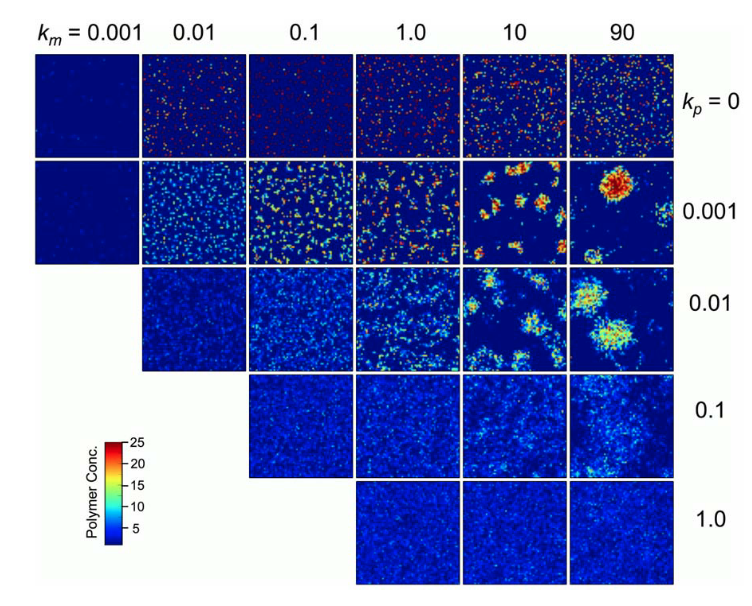
\includegraphics[width=0.75\textwidth]{figures/walker2012/fig3.png}
  \caption{Exploration of diffusivity parameters in \cite{walker_universal_2012}, illustrating spontaneous polymer aggregation.}
  \label{fig:walker2012fig3}
\end{figure}


\clearpage

\subsubsection{\texorpdfstring{\cite{fontana_what_1994}}{}}

\begin{markdown}

**tldr**; Using lambda-calculus to define an artificial chemistry system, the authors suggest that three invariants of evolution would inevitably reappear “if the tape were played twice”: hypercycles, self-sustaining organizations, more complex metaorganizations

- the authors develop an abstract chemistry implemented on lambda-calculus, and argue that the following features (that emerge in their model) arise generically: hypercycles, self-maintaining organizations, high-order self-maintaining organizations
    
- Gould: would the biodiversity that surrounds us be different if “the tape were played twice”, i.e. contingency vs necessity
    
- we can investigate this questions using a model—this model cannot assume the prior existence of organisms
    
- chemistry is based on the syntactic structure in which the molecules are assembled
    
- in lambda-calculus, objects are defined inductively in terms of a nonlinear combination of primitives
    
- this implies that each object is a function, such that we can write (A)B, or “the action of A on B”, which implies the “reduction in normal form” of (A)B --> C1 --> C2, …or, equivalently, (A)B=C
    
- lambda-calculus isn’t a theory of actual chemistry, e.g. no reference to thermodynamics—however TD driving is abstracted by requiring that every object is in normal form—or to spatial constraints, conservation laws, etc.
    
- the basic event in lambda-chemistry is a collision between two objects, happening inside a well-stirred flow reactor whose number of objects is kept constant
    
- level 0 experiments: 1000 random functions, one copy each—these experiments always become dominated by self-copying functions or hypercyclically coupled copying functions a la Eigen
    
- level 1 experiments: restricting copying functions generates complexity (see text and fig1) whose organizations are self-maintaining (instead of self-reproducing) and are very robust to perturbations (e.g., with random objects)
    
- level 2 experiments: initiated with the products of two level 1 experiments and have two outcomes, either a single level 1 organization dominates or a metaorganization arises with metabolic flows
    
- the results of these experiments can be summarized by three claims: hypercycles arise, when replication is prohibited complex self-maintaining organizations emerge, organizations can be hierarchically combined to produce new organizations
    
- the biological analogy to what precedes would be: the emergence of self-replication, self-maintaining prokaryotic organizations, self-maintaining eukaryotic organizations
    
- this challenges the view that Darwinian selection presupposes the existence of self-reproducing entities as these are absent from level 1-2
    
- this study also challenges the hypothetical, simultaneous emergence of self-reproduction and self-maintenance
	
\end{markdown}

\clearpage

\subsection{Assembly theory}

\subsubsection{\texorpdfstring{\cite{marshall_probabilistic_2017}}{}}

\begin{markdown}

**Summary:** Pathway Complexity is a (graph-based) method to measure the complexity of objects by calculating the number of steps required for their construction. It could be used as an agnostic biosignature, and to inform a new theory of biology.

- One thing that discriminates living systems is their ability to generate non-random structures in a large abundance—folded protein, lilving cells, microbial communities
    
- There’s been many proposals for finding biosignatures: gases (e.g., methane), Fe isotope ratio, biological impact on minerals, distribution in monomer abundance, red edge, etc.
    
- Two difficulties with biosignatures: casting our net wide enough (i.e., not remaining tied to terran biology) and avoiding false positives
    
- Prior definitions of complexity: Shannon entropy, Kolmogorov complexity, logical depth, effective complexity, computational complexity, stochastic complexity—but they sometimes give misleading results (e.g., maximal values for random structures)
    
- Pathway Complexity is a measure of complexity based on the construction of an object through joining operations of basic substructures, where the complexity is defined as the number of associated joining operations
    
- The reasoning behind Pathway Complexity is that objects of sufficient complexity would have their formation compete against the combinatorial explosion of possible objects—i.e., producing non-trivial construction trajectories would be a characteristic unique to life, which also makes the approach agnostic
    
- We can use a graph-based approach to evaluate the construction of objects
    
- There are both lower- and upper-bounds on the complexity of objects, and living systems produce objects that fall between these two extremes
    
- We can also use a variant called “recursive tree complexity” where we partition the object into subgraphs
    
- Pathway Complexity can be useful in the lab in exploring the threshold between living/non-living, and could inform a new theory for biology
    
\end{markdown}

\clearpage

\subsubsection{\texorpdfstring{\cite{marshall_identifying_2021}}{}}

\clearpage

\subsubsection{\texorpdfstring{\cite{marshall_formalising_2022}}{}}

\clearpage

\subsubsection{\texorpdfstring{\cite{jirasek_multimodal_2023}}{}}


\clearpage

\subsubsection{\texorpdfstring{\cite{sharma_assembly_2023}}{}}



\clearpage

\subsection{Topology of rock pores}

\subsubsection{\texorpdfstring{\cite{chogani_decoding_2023}}{}}

\begin{markdown}

**Summary:** Serpentinization of ultramafic rock exhibit nanoporosity that may—combined with a fractal network of pores—provide energy sources for the deep biosphere, change the physical properties of confined fluids and influence drastically the production of abiotic organics

- serpentinization of ultramafic rock exhibit nanoporosity that impact the geochemical behaviour ; can provide energy sources (e.g. H and CH4) for the deep biosphere
    
- here we investigate the characteristics, scale dependence and implications of nanoporosity
    
- using multidimensional imaging and molecular dynamics we conclude that serpentinites function as nanoporous media with pores < 100nm
    
- the fractale nature of pore size distribution support the presence of a nanoporous network with induces emergent properties in fluid transport, mineral solubility and chemical reactions
    
- while tectonic deformation and thermal cracking can generate fluid pathways in rocks, the mineral reaction itself can also induce differential stress causing the rock to fracture
    
- for this study samples representing the oceanic lithospheric mantle and exhumed mantle on land were collected through the Ocean Drilling Program at the Mid-Atlantic Ridge and in an ultramafic complex in Norway—both samples are composed of lizardite
    
- there is currently an absence of a robust model that elucidates the genesis of nanoporosity in serpentinites
    
- analysis reveals that serpentine pores are generally elongated rather than circular—which may be attributed to the underlying mineral formation process
    
- moreover, pore size distribution exhibits fractal characteristics—suggesting that pores at various scales can be attributed to the same underlying processes
    
- serpentinites function as nanoporous media with pores of less than 100nm—fluid restricted to these scales exhibit distinct behaviours which could influence fluid and mass transport or change the physical properties of the fluid—molecular dynamics simulations suggest that the reduction of CO2 to CH4 is favoured in these conditions, possibly having drastic effects on e.g. the production of abiotic organics
    
\end{markdown}

\clearpage

\subsubsection{\texorpdfstring{\cite{tallarek_probing_2023}}{}}

\begin{markdown}

**Summary:** Investigates, using molecular dynamics and Brownian dynamics simulations, the behaviour of chemicals passing moving through porous media and the impact of the environment on molecular diffusion. Concludes that chain length and density, as well as type of molecule, influence diffusion the most.

- This study investigates how chemicals move through porous media, which can have complex structures—and can impact molecular diffusion
    
- Integrates molecular dynamics simulations to investigate the dynamics at the mesopore level
    
- Integrates Brownian dynamics simulations to investigate diffusion at the mesopore and macropore levels
    
- Chain length and density greatly influence diffusion coefficients
    
- The effective diffusion coefficients were more influenced by the type of molecule than by the surface chemistry
    
- These results have implications in designing chromatographic materials, and optimizing separation processes in various fields (pharmaceuticals, environmental engineering, etc.)

\end{markdown}

\clearpage

\subsubsection{\texorpdfstring{\cite{walker_life_2024}}{}}

\begin{markdown}

**Chapter 1: what is life?**

- 7: does “life” exist? is it a property of the parts? can it be explainable by the known laws of physics and chemistry?
- 11: there is no “magic transition point” where a (collection of) molecule is suddenly living
- 26: instead of answering “what is life?” we might have to transition to answering “why life?” and similarly go from defining life to deriving life’s properties from a (new) fundamental physical theory
- 29: biologists are too focused on defining life in terms of features observed on Earth, astrobiologists are too anthropocentric too, chemists think it’s all chemistry, computer scientists only focus on the software, physicists focus on thermodynamics, etc.

**Chapter 2: hard problems**

- 32: three fundamental problems for science: origins of matter, life, mind
- 40: in order to test a theory, it must have measurable consequences on the world
- 44: focusing on chemical correlates (e.g.: compartmentalization) has, after decades, yielded only limited progress—are we missing something more fundamental? we need new physics: “how is it that information can cause things?”
- 53: the three hard problems can be framed as “why do some things exist and not others?”

**Chapter 3: life is what?**

- 70: we have not yet built a physics that deals with the combinatorial space of all possible objects that can be built from elementary stuff
- 71: in order to explain these objects, we have to reconceptualize the space of combinatorial possibilities as a physical space
- 73: we have to formalize the foundations of a theory for life not in terms of what life is, but of what life does—as life is the only thing in the universe that can make objects that are composed of many unique, recursively constructed parts
- 74: the key hypothesis of assembly theory is that the observation of complex objects implies that the “information” about the steps of their formation must exist in other objects (implies a physically instantiated memory) which can happen only via evolution or learning—if selection acts as a constraint that can drive the emergence of life, we need to discover the laws of physics that explain selection
- 75: current physics puts all causation at the microscale, whereas in assembly theory almost no causation exists in elementary objects—causation is built up over time along lineages
- 76: the copy number—how many of a given object you observe—is of fundamental importance in defining a theory that accounts for selection, as the more parts it has the less likely an exact copy can exist without some precise mechanism that has itself been selected generates the object
- 78: the assembly index is the way we formalize how hard it is for the universe to build something—defined by the smallest number of physically possible steps necessary to produce an object—the assembly space captures the minimal memory, in terms of the minimal number of operations necessary to assembly the observed object, based on objects that could have existed in its past
- 84: the minimal path in assembly theory is agnostic and does not depend on the chemistry of life as we know it, we can go in the lab and measure it using several different instruments, and for any molecule
- 87: distinguishing design (via an intelligent agent or an evolutionary process) from randomness is important in the context of detecting alien intelligences in the universe, via the signatures of their technology
- 88: the idea of comploxity peak goes back to earlier work in complex systems, including that of Jim Crutchfield and colleagues demonstrating how a peak in complexity somewhere between fully ordered and totally random (high entropy) characterizes the behavior of many systems
- 95: most of the excitement around what we are doing with assembly theory has so far focused on how it provides the first theoretically motivated and empirically tested solution to the problem of ruling out false positives in alien life detection
- 97: we need to define a threshold assembly index and copy number that determines when an object must have been produced by a causal chain of stacked objects, meaning life
- 97: to make an alien life-detection system, the first step was to confirm that assembly index can be measure with laboratory instrumentation—what Lee’s lab found is that the assembly index of a molecule correlates directly with features of the fragmentation pattern of the molecule
- 99: assembly index is an intrinsic property of a molecule—it is a feature we can find via a multimodal suite of different measuring techniques (infrared spectroscopy and nuclear magnetic resonance)
- 99: what we observed experimentally is that this threshold in chemical space for observing objects made by life (and only life) is fifteen steps (for the chemical space on Earth at least
- 100: fifteen is about where we hit the threshold of one copy per mole without selection
- 101: work done in Sara’s lab aims to refine the theory around this threshold as a phase transition in the possibility of objects existing (carried out by Dániel Czégel, Gage Seibert, and Swanand Khanapurk

**Chapter 4: aliens**

- “NASA started investing more concretely in astrobiology research, founding shortly thereafter the NASA Astrobiology Institute (NAI). Over its twenty years in operation between 1998 and 2019, the NAI launched many of astrobiology’s most important research agendas and fostered a new generation of scientists tackling the open questions of astrobiology. In 2017, the annual NASA Space Act declared the search for alien life among the primary objectives of NASA for the first time in history. Astrobiology is now a major theme throughout several NASA mission directorates” (Walker, 2024, p. 119)
- “A fundamental understanding of life will begin a new era of astrobiology, because it will allow us to move beyond the search for life as one of analogy. It will allow us to search for life as we don’t know it. Indeed, it will allow us to search for life as no one knows it. Understanding life in the abstract will allow us to predict what alien examples of life could be like. Our hope with assembly theory is that we will be able to use it to detect alien life, if it is out there, and that even before we make first contact we also might use it to predict features of the possibility spaces aliens might live in.” (Walker, 2024, p. 128)
- “As my geochemistry colleagues at Arizona State University Everett Shock and Hilairy Hartnett advocate, “Biochemistry is what the Earth allows.”[5] (Walker, 2024, p. 129)
- “consider all of the microenvironments across a planetary surface as microreactors, and a planet as an engine exploring via these microenvironments the combinatorial space of geochemically possible small molecules.[7] Fluctuations in the density of assembly happen, and life emerges as a cascade of objects building into the high assembly universe.” (Walker, 2024, p. 131)
- “When we can run origin-of-life experiments at scale, they will allow us to predict how much variation we should expect in different geochemical environments. That is, we will not only be able to speculate that life elsewhere should be different, but we should be able to say how different with quantitative precision.” (Walker, 2024, p. 133)
- “A very different sense of universality, found in physics, could be useful for guiding our search for alternative forms of life. That concept arises from the study of phase transitions. Familiar examples of phase transitions include when ice melts or when liquid water vaporizes. Physicists refer to the physical conditions where a phase transition occurs as a critical point. In the study of phase transitions, an important mathematical tool has been the identification of scaling laws, which allow the quantification of the systematic variation of one property with another—for example, how temperature might scale with pressure. Universality classes in physics are then identified by systems that have the same scaling behavior.[11] Remarkably, this can occur across systems that are completely different in terms of their component parts and microscopic physics: the water-gas phase transition has the same scaling behavior as the one that occurs in magnetic materials between the ordered and disordered phases (where magnets align or point in random directions respectively). Physicists have used this to predict properties of new materials that might be in the same universality class as existing ones—e.g., share the same macroscale properties (scaling) while varying in lower-level microscopic detail (whether the system is made of water or a magnetic material). This offers the possibility that scaling laws identified for life’s chemistry might enable us to predict features of alien chemistry. The first challenge is to determine if generalizable trends indeed do exist.” (Walker, 2024, p. 134)
- “There are two resolutions to the challenges of life detection I’ve posed. Either we need biosignatures that are not subject to false positives, or we need to determine the probability for an origin-of-life event. Assembly theory solves the problem of false positives, because a falsifiable hypothesis of the theory is that life is the only mechanism that can produce high assembly objects.” (Walker, 2024, p. 148)
- “we are currently working on getting assembly theory “flight-ready” by calculating how feasible it is to make a detection of high assembly molecules using current mass-spec instrumentation from prior and upcoming NASA missions. This could prove critically important for analyzing data from solar system worlds like Titan, which the NASA Dragonfly mission will visit in the coming decades.” (Walker, 2024, p. 148)

**Chapter 5: origins**

- “That conversation marked the beginning of our moon-shot project to solve the origin of life and first contact with alien life at the same time. We are going to need a very large experiment for this one. Planets are not easy to simulate with physical material, but this is not a simulation we can run in a computer. We would not even know what to program into a simulation, because we don’t know how chemistry generates life.” (Walker, 2024, p. 153)
- “We must build a physical experiment to simulate planetary conditions to search for the origin of alien life for a similar reason. We need to test our theories against reality, and we can do so only in experiments that can explore the high combinatorial diversity of the chemical universe.” (Walker, 2024, p. 154)
- “How then can we design an experiment and expect to observe the spontaneous emergence of life, e.g., via the spontaneous emergence of design we did not put in? The boundaries of any experiment we make to produce an origin-of-life event will always be set by information and constraints that are themselves the product of an origin-of-life event. This problem is not widely discussed in the origin-of-life literature, but it should be. My collaborators and I are aiming to get ahead of it by identifying how to quantify our agency and the informational constraints we impose on chemistry when we do origin-of-life experiments. We need to do this if we are to solve how life happens without us. To do so, we need to make an information vacuum” (Walker, 2024, p. 157)
- “Because the chemputer has digitized chemistry—it runs explicitly on an algorithmic procedurewe can precisely quantify how much information we are putting into the experiment. Because we have assembly theory, we can quantify the assembly of the starting molecules and track how assembled things become over time to look for evidence of the emergence of evolution and selection within the boundary conditions of the experiment. These two things when combined allow us to quantify how much of an “information vacuum” we have created via the experiment itself being a part of a lineage of life, versus how much assembly the chemistry in the experiment generates de novo.” (Walker, 2024, p. 169)

**Chapter 6: planetary futures**

\end{markdown}

\clearpage

\section{References}
%\bibliographystyle{apalike}
\footnotesize
\setlength{\bibsep}{0.0pt}
\bibliography{references-new.bib}

\end{document}
